\documentclass[]{article}

\usepackage[utf8]{inputenc}
\usepackage{amsmath}
\usepackage{amssymb}
\usepackage{amsthm}
\usepackage{amsfonts}
\usepackage{graphicx}
\usepackage{capt-of}
\usepackage{listings}
\usepackage{siunitx}
\usepackage[section]{placeins}
\usepackage{float}
\usepackage{caption}
\usepackage{subcaption}



% Oppgavenummerering %
\renewcommand\thesection{Task \arabic{section}}
\renewcommand\thesubsection{\alph{subsection})}
\renewcommand\thesubsection{\alph{subsection})}

% Bevis
\newcommand\TombStone{\rule{.5em}{.5em}}
\renewcommand\qedsymbol{\TombStone}
\renewcommand{\proofname}{Bevis.} % Norske bevis

\title{TDT4195 - IP Assignment 2}
\author{Sigurd Totland | MTTK}

\begin{document}
\maketitle

\section{CNN Theory}
\subsection{}
From equation (1) in the assignment,
\begin{equation}\begin{aligned}
W_2 = \frac{W_1 - F_W + 2 P_W}{S_W} + 1,
\end{aligned}\end{equation}
we get that the padding $P_W$ should be
\begin{equation}\begin{aligned}
P_W = \frac{1}{2}(S_W W_2 - W_1 + F_W - S_W).
\end{aligned}\end{equation}
Since we want the output image to have equal dimensions to the input, we require $W_2 = W_1$. Furthermore, we are given stride $S_W = 1$ and filter width $F_W = 5$, which yields
\begin{equation}\begin{aligned}
P_W = \frac{1}{2}(W_1 - W_1 + 5 - 1) = 2.
\end{aligned}\end{equation}
Since the filter is square, the horisontal and vertical padding is identical.

\section{CNN Programming}
\subsection{Maxpooling}
When maxpooling is applied to Chelsea, we get the result in figure \ref{fig:chelsea}.
\begin{figure}[H]
     \centering
     \begin{subfigure}[b]{0.6\textwidth}
         \centering
         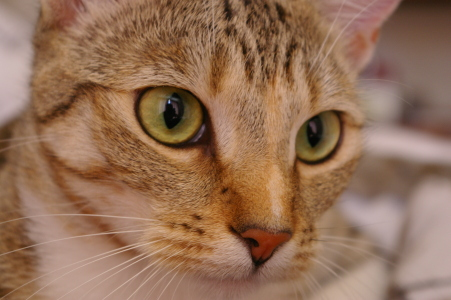
\includegraphics[width=\textwidth]{chelsea}
         \caption{Original Chelsea}
         \label{fig:chelsea_before}
     \end{subfigure}
     \hfill
     \begin{subfigure}[b]{0.3\textwidth}
         \centering
         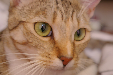
\includegraphics[width=\textwidth]{chelsea_maxpooled}
         \caption{Post-maxpool Chelsea}
         \label{fig:chelsea_after}
     \end{subfigure}
    \caption{Chelsea before and after maxpooling}
    \label{fig:chelsea}
\end{figure}
The checkerboard has 2x2 checkers, meaning that the maxpooled image is simply a white square, as shown in figure \ref{fig:checkerboard}.
\begin{figure}[H]
     \centering
     \begin{subfigure}[b]{0.6\textwidth}
         \centering
         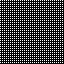
\includegraphics[width=\textwidth]{checkerboard}
         \caption{Original board}
         \label{fig:checkerboard_before}
     \end{subfigure}
     \hfill
     \begin{subfigure}[b]{0.3\textwidth}
         \centering
         
\includegraphics[width=\textwidth]{checkerboard_maxpooled}
         \caption{Post-maxpool board}
         \label{fig:checkerboard_after}
     \end{subfigure}
    \caption{Chelsea before and after maxpooling}
    \label{fig:checkerboard}
\end{figure}


\subsection{CNN MNIST Classifier}
Implementing the CNN form Table 1 in the assignment and training it on the MNIST dataset yields final training loss of $0.044$ and $99\%$ accuracy(!). The plot of loss is shown in figure \ref{fig:task2} below.
\begin{figure}[H]
\centering
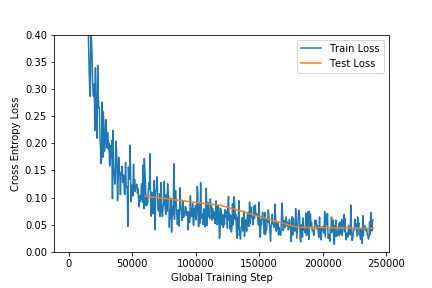
\includegraphics[width=0.7\textwidth]{task2}
\caption{Training loss of 4 epochs}
\label{fig:task2}
\end{figure}
From figure \ref{fig:task2}, we do not see evidence of overfitting with these hyperparameters, as the test loss and final test accuracy corresponds well with the training loss. Had the test loss been significantly worse than the training loss however, one would suspect the network to be overfitted to the training data.

\subsection{}
When trained for 10 epochs instead of two, the training loss develops like shown in figure \ref{fig:task2_10epochs} below.
\begin{figure}[H]
\centering
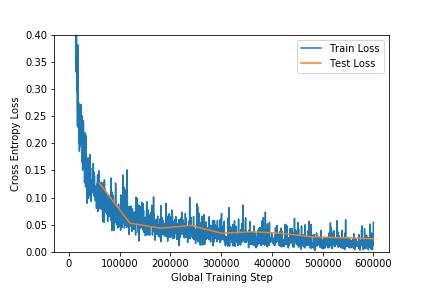
\includegraphics[width=0.7\textwidth]{task2_10epochs}
\caption{Training loss of 10 epochs}
\label{fig:task2_10epochs}
\end{figure}
This time, the final validation accuracy is $99.1\%$ and the final validation loss is $0.024$. Again, we do not see evidence of overfitting as the test loss and training loss still correspond.

\subsection{}
We plot the weights numbered 5, 8, 19, 22, and 34 in the first convolutional layer of ResNet50 along with the corresponding activation on the input zebra image. These results are shown in \ref{fig:zebra_activation} below.
\begin{figure}[H]
\centering
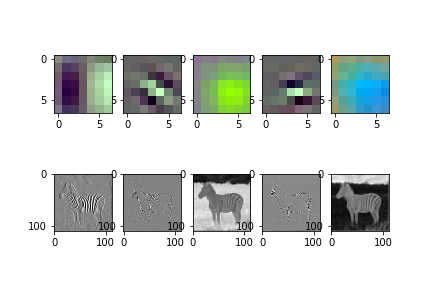
\includegraphics[width=0.7\textwidth]{zebra_activation}
\caption{ResNet50 weights and corresponding activation on zebra image}
\label{fig:zebra_activation}
\end{figure}

\subsection{}
We see, as expected, how the filters more strongly activate those parts of the image that they are supposed to. The first filter for instance, resembles a simple edge detection filter although widened a bit, and indeed it brings out the stripes of the zebra the most, in addition to applying a light edge detection on the entire zebra. The second filter looks like a sobel as well, but it is rotated. Note how it does not bring out the zebra stripes by a lot, but it does apply some edge detection, especially on the edges of the zebra with similar orientation to it. The third filter is green and smooth, and seems to bring out the smooth grass background. For the fourth filter we have yet another, this time horisontal, edge detector. Notice how it does not activate on the vertical stripes of the zebra at all, and activates almost exclusively in the areas where the stripes are horisontal. Lastly, we have an almost entirely smooth, blue filter, which unsurprisingly brings out the smooth, blue sky.

\section{Frequency Domain Filtering Theory}
\subsection{}
To perform the convolution $f * g$ using the convolution theorem, we
\begin{enumerate}
\item take the Fourier transform of $f$ and $g$,
\item multiply the transformed functions, obtaining $\mathcal{F}\{f*g\} = \mathcal{F}\{f\} \cdot \mathcal{F}\{g\}$,
\item inverse transform the result, obtaining $f * g = \mathcal{F}^{-1}\{\mathcal{F}\{f*g\}\}$.
\end{enumerate}

\subsection{}
High pass filters damp the lowest frequencies of a function and preserves high-frequency components. Low pass filters do the opposite and damp the highest frequencies, such as noise, while preserving slow dynamics.

\subsection{}
The filter in a) corresponds to a high pass filter, but only in the vertical direction. In the horisontal, it damps all frequencies, also high ones. The filter in b) is a high pass filter – the center (low frequencies) are damped and the outer region is preserved. The final filter in c) is a low pass filter as only center frequencies (low frequencies) are preserved.

\section{Frequency Domain Programming}
\subsection{}
We implement kernel convolution via the frequency domain using the convolution theorem. Applying a high pass filter on the \texttt{skimage.data.camera()} camera man image, we get the results shown in figure \ref{fig:cameraman_hp}.
\begin{figure}[H]
\centering
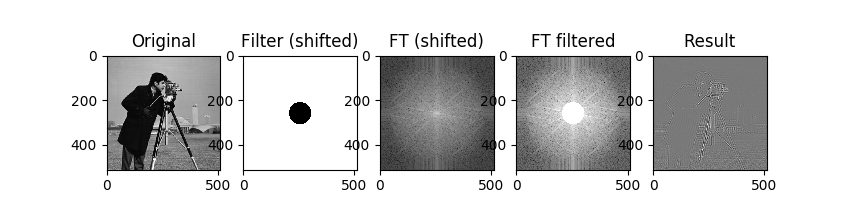
\includegraphics[width=\textwidth]{camera_hp_verbose}
\caption{Camera man high pass filtered}
\label{fig:cameraman_hp}
\end{figure}
Applying a low pass filter on the same image results in the results in figure \ref{fig:cameraman_lp} below.
\begin{figure}[H]
\centering
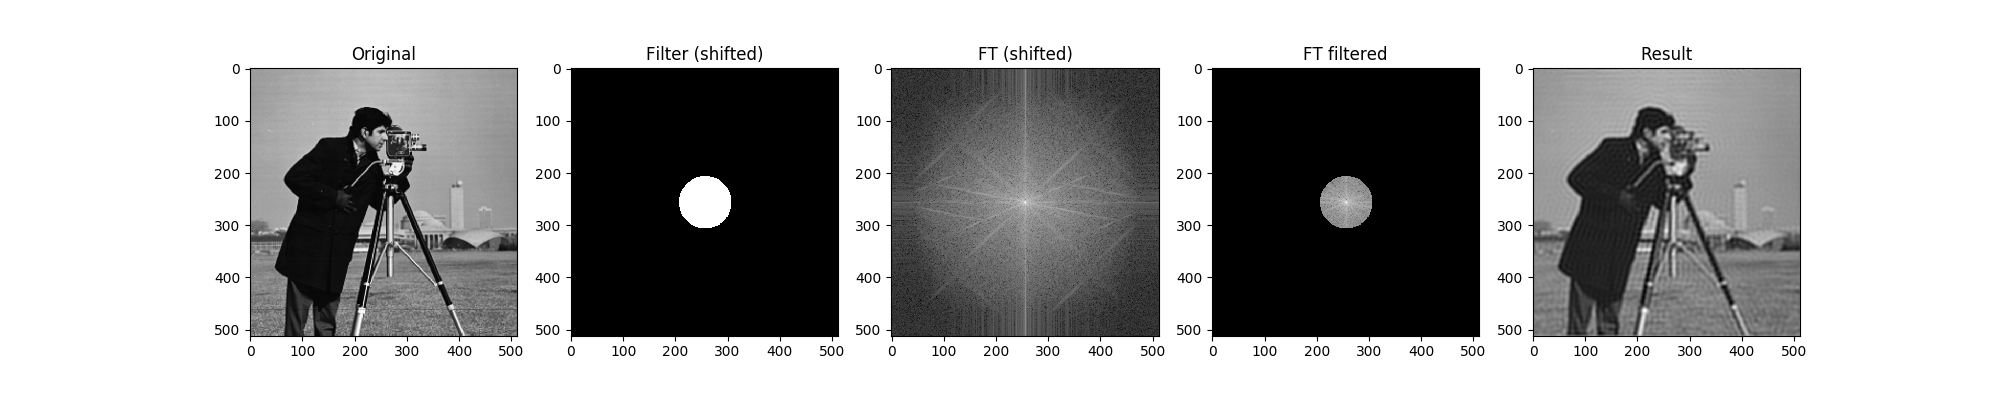
\includegraphics[width=\textwidth]{camera_lp_verbose}
\caption{Camera man low pass filtered}
\label{fig:cameraman_lp}
\end{figure}

\subsection{}
In this task we implement kernel convolution through the frequency plane. We must then pad the input kernel in the bottom left corner to match the dimensions of the input image before taking the Fourier transform. With a gaussian kernel, we get the results shown in figure \ref{fig:camera_gauss} below.
\begin{figure}[H]
\centering
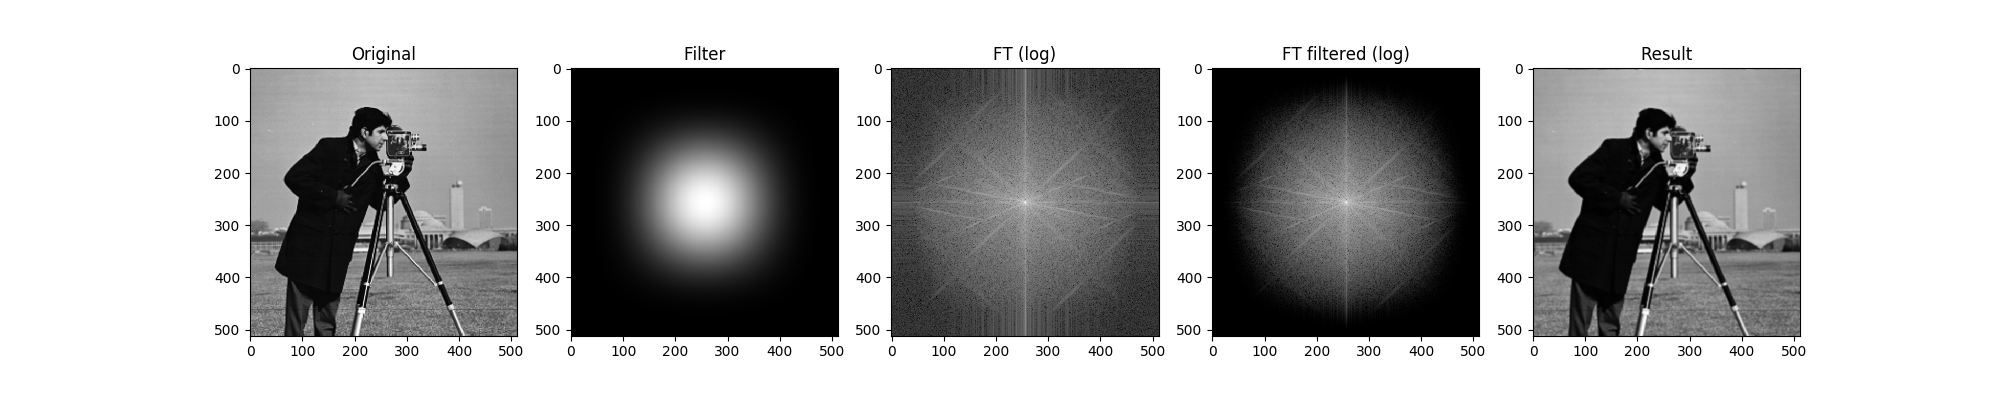
\includegraphics[width=\textwidth]{camera_gauss}
\caption{Camera man gaussian blurred in frequency domain}
\label{fig:camera_gauss}
\end{figure}
Applying a 3-by-3 sobel in the x-direction with the same methods yields the results in figure \ref{fig:camera_sobel}.
\begin{figure}[H]
\centering
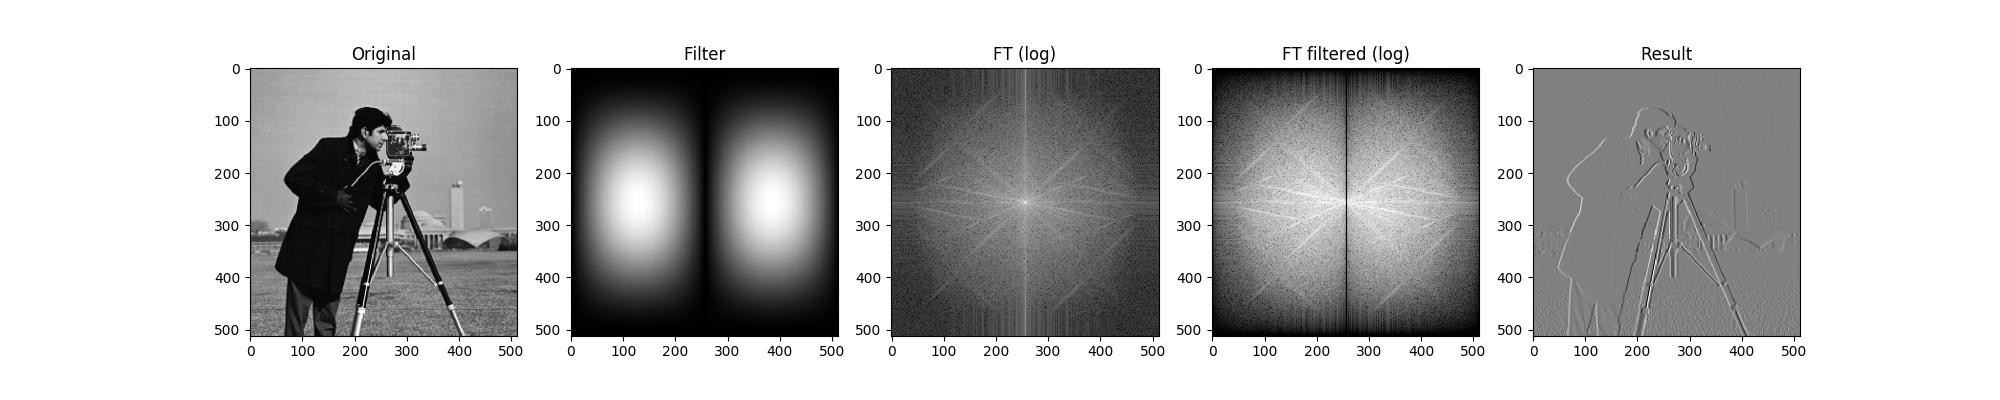
\includegraphics[width=\textwidth]{camera_sobel}
\caption{Camera man with sobel filter applied in the frequency domain}
\label{fig:camera_sobel}
\end{figure}
Larger scale versions of the two processed images are shown in figure \ref{fig:processed_freq}.

\begin{figure}[H]
     \centering
     \begin{subfigure}[b]{0.45\textwidth}
         \centering
         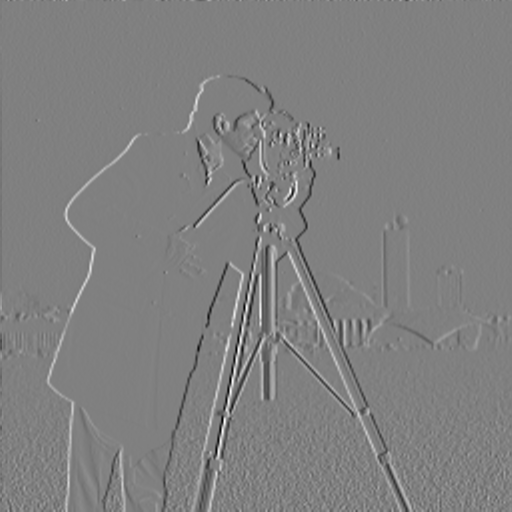
\includegraphics[width=\textwidth]{camera_sobelx}
         \caption{Sobel result}
         \label{fig:sobel_after}
     \end{subfigure}
     \hfill
     \begin{subfigure}[b]{0.45\textwidth}
         \centering
         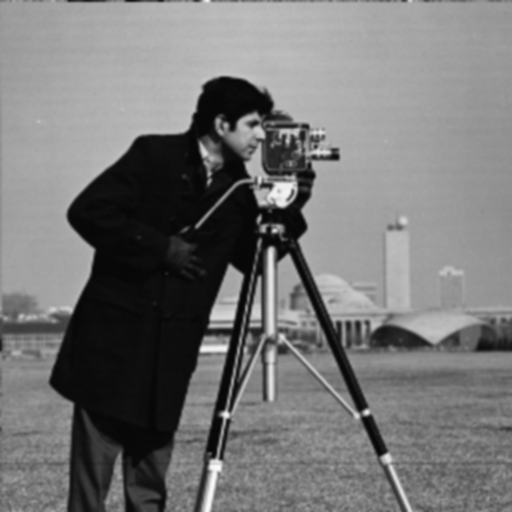
\includegraphics[width=\textwidth]{camera_gaussian}
         \caption{Gaussian blur result}
         \label{fig:gauss_after}
     \end{subfigure}
    \caption{Images processed in the frequency domain}
    \label{fig:processed_freq}
\end{figure}

\subsection{}
We apply the notch filter to the clown image. The results of this can be seen in figure \ref{fig:clown_results}.
\begin{figure}[H]
\centering
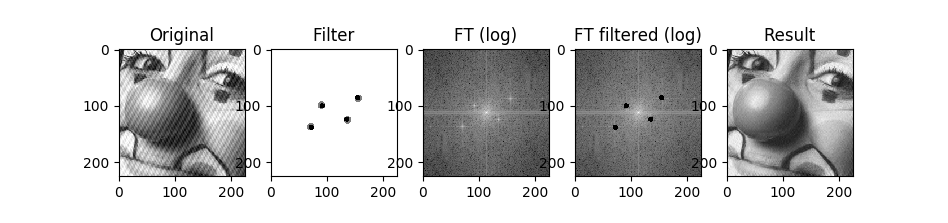
\includegraphics[width=\textwidth]{clown_results}
\caption{Clown filter results}
\label{fig:clown_results}
\end{figure}
Full size before and after images for the clown image, which clearly shows the periodic pattern present in the original image, and that it is removed almost entirely (except around the edges of the image) in the filtered image are shown in figure \ref{fig:clown_before_after}.
\begin{figure}[H]
     \centering
     \begin{subfigure}[b]{0.45\textwidth}
         \centering
         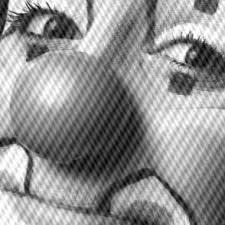
\includegraphics[width=\textwidth]{clown}
         \caption{Original}
         \label{fig:clown_orig}
     \end{subfigure}
     \hfill
     \begin{subfigure}[b]{0.45\textwidth}
         \centering
         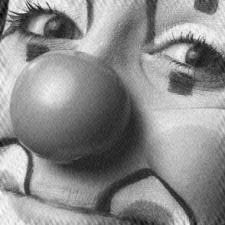
\includegraphics[width=\textwidth]{clown_filtered}
         \caption{Notch filtered}
         \label{fig:clown_filtered}
     \end{subfigure}
    \caption{Clown image before and after notch filtering}
    \label{fig:clown_before_after}
\end{figure}
The filter used here is an example of a notch filter. A notch filter damps a specific frequency range in the signal, which makes it the ideal tool to remove unwanted periodic patterns in an image, such as the pattern overlayed on the clown image. Looking at the Fourier transform of the input image, we can see four bright spots which correspond to the unwanted pattern. A notch filter can then be specifically crafted to eliminate the pattern from the image.




\end{document}

